

\tikzset{every picture/.style={line width=0.75pt}} %set default line width to 0.75pt        

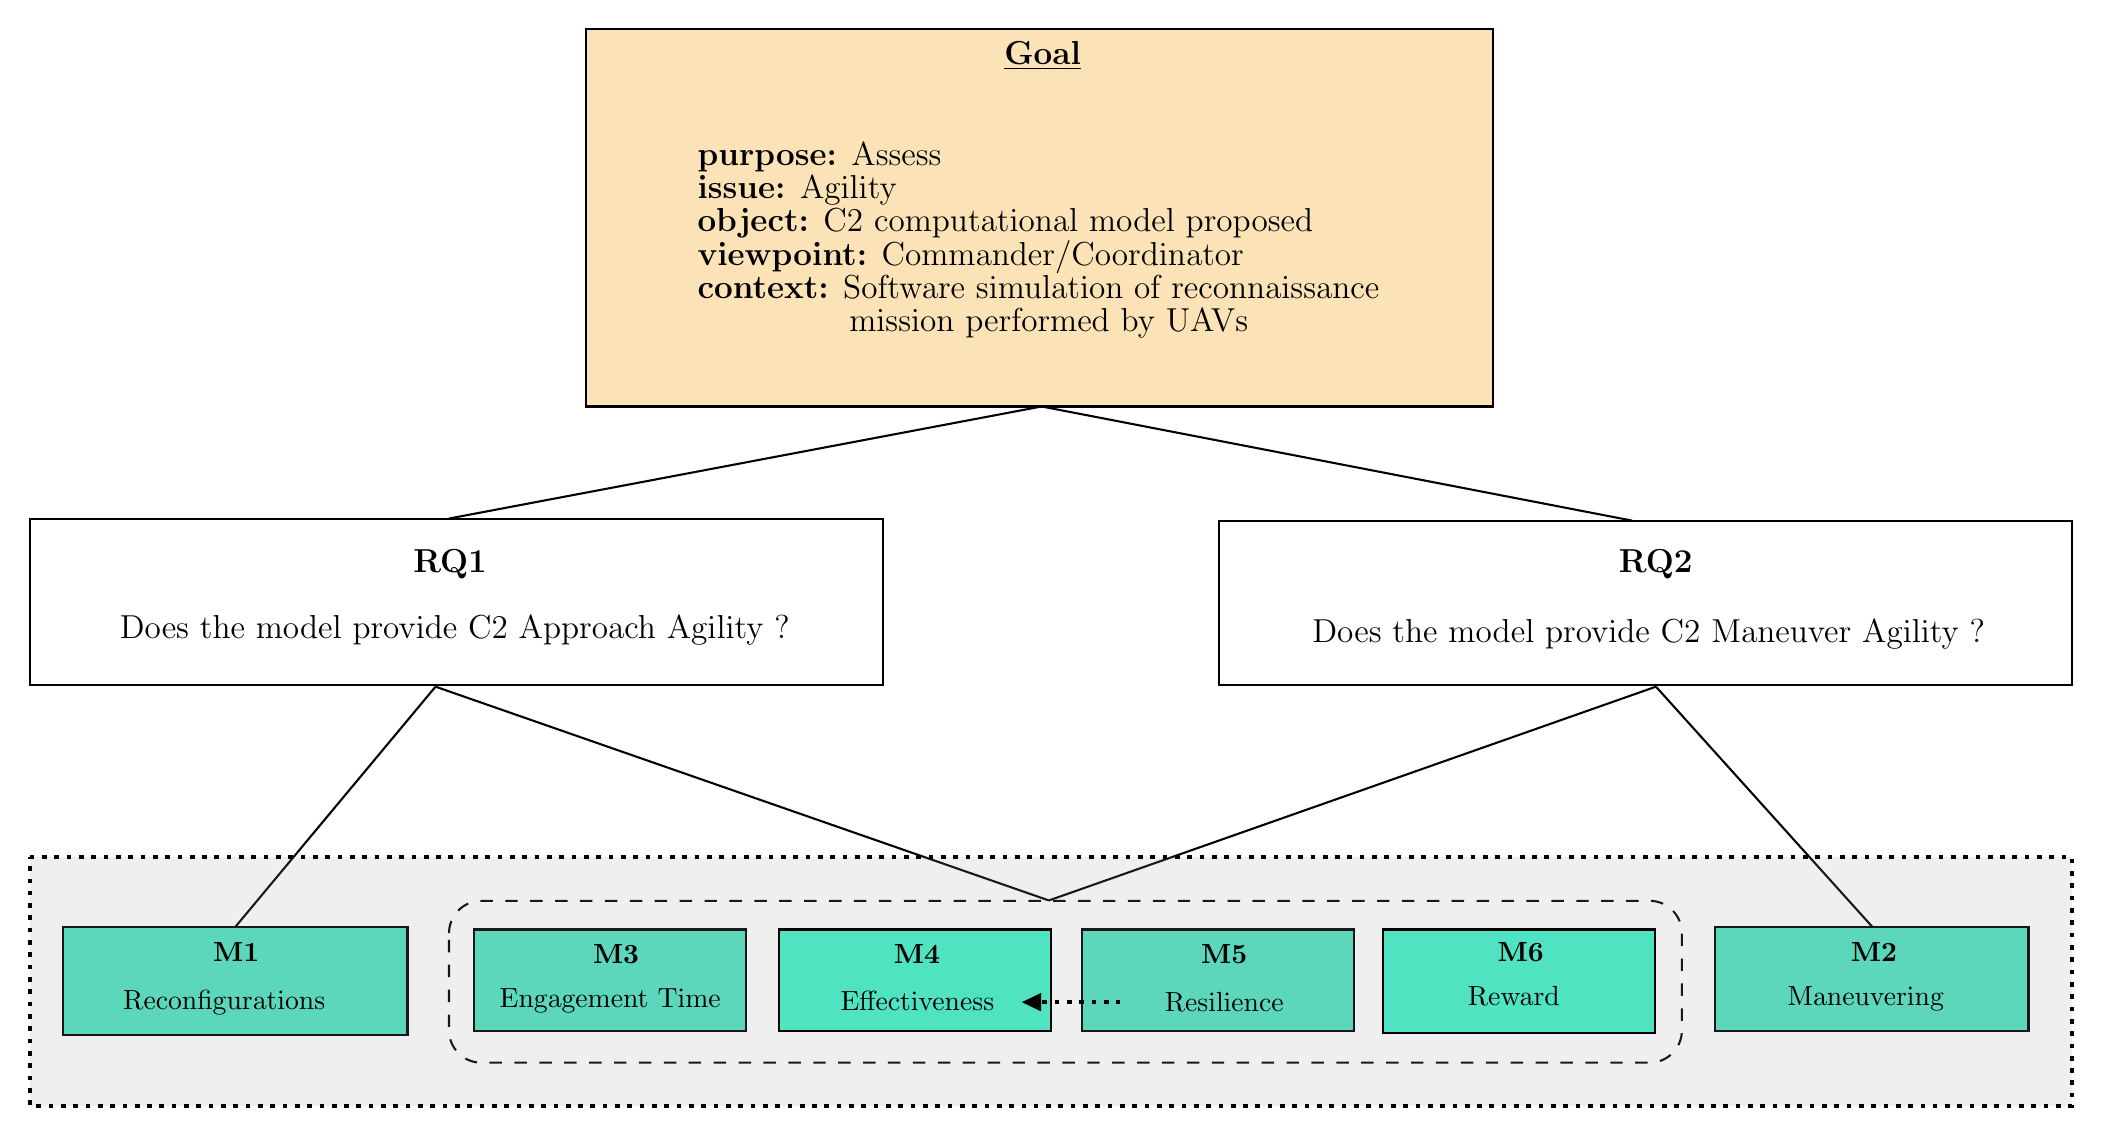
\begin{tikzpicture}[x=0.75pt,y=0.75pt,yscale=-1,xscale=1]
%uncomment if require: \path (0,532); %set diagram left start at 0, and has height of 532

%Flowchart: Process [id:dp9228173025001839] 
\draw  [fill={rgb, 255:red, 245; green, 166; blue, 35 }  ,fill opacity=0.33 ] (286.5,2) -- (723.5,2) -- (723.5,184) -- (286.5,184) -- cycle ;
%Shape: Rectangle [id:dp9468174970136011] 
\draw   (591.5,239) -- (1002.5,239) -- (1002.5,318) -- (591.5,318) -- cycle ;
%Shape: Rectangle [id:dp09665993774558346] 
\draw   (18.5,238) -- (429.5,238) -- (429.5,318) -- (18.5,318) -- cycle ;
%Straight Lines [id:da1961523796551078] 
\draw    (506,184) -- (220.5,238) ;
%Straight Lines [id:da6120336423295578] 
\draw    (506,184) -- (790.5,239) ;
%Shape: Rectangle [id:dp8704718643302001] 
\draw  [fill={rgb, 255:red, 80; green, 227; blue, 194 }  ,fill opacity=1 ] (232.5,436) -- (363.5,436) -- (363.5,485) -- (232.5,485) -- cycle ;
%Rounded Rect [id:dp2310824766673354] 
\draw  [dash pattern={on 4.5pt off 4.5pt}] (220.5,437.77) .. controls (220.5,429.15) and (227.48,422.17) .. (236.1,422.17) -- (798.9,422.17) .. controls (807.52,422.17) and (814.5,429.15) .. (814.5,437.77) -- (814.5,484.57) .. controls (814.5,493.18) and (807.52,500.17) .. (798.9,500.17) -- (236.1,500.17) .. controls (227.48,500.17) and (220.5,493.18) .. (220.5,484.57) -- cycle ;
%Straight Lines [id:da04635172987230718] 
\draw    (214,319) -- (116.5,436) ;
%Shape: Rectangle [id:dp16323070417268737] 
\draw  [fill={rgb, 255:red, 80; green, 227; blue, 194 }  ,fill opacity=1 ] (34.5,435) -- (200.5,435) -- (200.5,487) -- (34.5,487) -- cycle ;
%Straight Lines [id:da004791401702264886] 
\draw    (214,319) -- (509.5,422) ;
%Straight Lines [id:da9733307686397392] 
\draw    (802,319) -- (509.5,422) ;
%Straight Lines [id:da4492045519053316] 
\draw    (802,319) -- (906.5,435) ;
%Shape: Rectangle [id:dp7181001754521874] 
\draw  [fill={rgb, 255:red, 80; green, 227; blue, 194 }  ,fill opacity=1 ] (830.5,435) -- (981.5,435) -- (981.5,485) -- (830.5,485) -- cycle ;
%Shape: Rectangle [id:dp46797453967825375] 
\draw  [fill={rgb, 255:red, 80; green, 227; blue, 194 }  ,fill opacity=1 ] (525.5,436) -- (656.5,436) -- (656.5,485) -- (525.5,485) -- cycle ;
%Rounded Rect [id:dp9444454858651523] 
\draw  [fill={rgb, 255:red, 155; green, 155; blue, 155 }  ,fill opacity=0.16 ][dash pattern={on 1.69pt off 2.76pt}][line width=1.5]  (18.5,401) .. controls (18.5,401) and (18.5,401) .. (18.5,401) -- (1002.5,401) .. controls (1002.5,401) and (1002.5,401) .. (1002.5,401) -- (1002.5,521) .. controls (1002.5,521) and (1002.5,521) .. (1002.5,521) -- (18.5,521) .. controls (18.5,521) and (18.5,521) .. (18.5,521) -- cycle ;
%Shape: Rectangle [id:dp6205174536004793] 
\draw  [fill={rgb, 255:red, 80; green, 227; blue, 194 }  ,fill opacity=1 ] (379.5,436) -- (510.5,436) -- (510.5,485) -- (379.5,485) -- cycle ;
%Straight Lines [id:da0036921302300286785] 
\draw [line width=1.5]  [dash pattern={on 1.69pt off 2.76pt}]  (500.5,471) -- (544,471) ;
\draw [shift={(496.5,471)}, rotate = 0] [fill={rgb, 255:red, 0; green, 0; blue, 0 }  ][line width=0.08]  [draw opacity=0] (9.29,-4.46) -- (0,0) -- (9.29,4.46) -- cycle    ;
%Shape: Rectangle [id:dp36331169023965726] 
\draw  [fill={rgb, 255:red, 80; green, 227; blue, 194 }  ,fill opacity=1 ] (670.5,436) -- (801.5,436) -- (801.5,486) -- (670.5,486) -- cycle ;

% Text Node
\draw (506.5,15) node  [font=\normalsize] [align=left] {\textbf{\underline{{\large Goal}}}};
% Text Node
\draw (221,260) node   [align=left] {\textbf{{\large RQ1}}};
% Text Node
\draw (223.25,292) node   [align=left] {{\large Does the model provide C2 Approach Agility ?}};
% Text Node
\draw (798.5,293.5) node   [align=left] {{\large Does the model provide C2 Maneuver Agility ?}};
% Text Node
\draw (801.92,260) node   [align=left] {\textbf{{\large RQ2}}};
% Text Node
\draw (504.5,104) node   [align=left] {{\large \textbf{purpose:} Assess}\\{\large \textbf{issue:} Agility}\\{\large \textbf{object:} C2 computational model proposed}\\{\large \textbf{viewpoint:} Commander/Coordinator}\\{\large \textbf{context:} Software simulation of reconnaissance }\\{\large  \ \ \ \ \ \ \ \ \ \ \ \ \ \ mission performed by UAVs}};
% Text Node
\draw (301,448) node   [align=left] {\textbf{M3}};
% Text Node
\draw (118,447) node   [align=left] {\textbf{M1}};
% Text Node
\draw (907,447) node   [align=left] {\textbf{M2}};
% Text Node
\draw (298.17,470.17) node   [align=left] {Engagement Time};
% Text Node
\draw (594,448) node   [align=left] {\textbf{M5}};
% Text Node
\draw (446.17,470.17) node   [align=left] {Effectiveness};
% Text Node
\draw (446,448) node   [align=left] {\textbf{M4}};
% Text Node
\draw (594,471) node   [align=left] {Resilience};
% Text Node
\draw (62,464) node [anchor=north west][inner sep=0.75pt]   [align=left] {Reconfigurations};
% Text Node
\draw (864,462) node [anchor=north west][inner sep=0.75pt]   [align=left] {Maneuvering};
% Text Node
\draw (736.87,447) node   [align=left] {\textbf{M6}};
% Text Node
\draw (709.87,462) node [anchor=north west][inner sep=0.75pt]   [align=left] {Reward};


\end{tikzpicture}